\section{Implementation and Results}
The framework of our system is implemented with Python with Scikit-learn library for dimension reduction and clustering.
As we are currently working with data with reduced size, the data are locally stored in the hard disk of an local workstation.
All the computation are undertaken by one core of a Intel Core i5 3.2 Ghz quad processor.
As we are aiming at identify and visualize similar climate patterns for the current milestone, we do not have any annotated groundtruth from the dataset.
In order to achieve sanity check for our algorithms and prepare for the comming large-scale experiment, we use an ambiguious but effective measure.
More specifically, we verify the result with our prior geology knowledge. E.g. we verify whether different clusters are constructed along China's coastal and inland areas.
In the following subsection, we will first analyse clustering and visualization results for different continents.
Extended discussion about parameters in clustering and dimension reduction algorithms will follow with concrete examples.

\subsection{Clustering Result Verification}
When verifying the results with our prior geology knowledge, we use 60 dimensional mean-value-based feature with 75 cluster components for North American continent and with 50 cluster components for Asia. We use different cluster numbers to better illustrate the results as the intrinsic climate patterns are different on the two continents. 
                    
\begin{figure}
    \centering
    \begin{tabular}{c c}
        \includegraphics[width=.45\linewidth]{./figure/Ave_60_comp_75_clu_USA.png}
        & 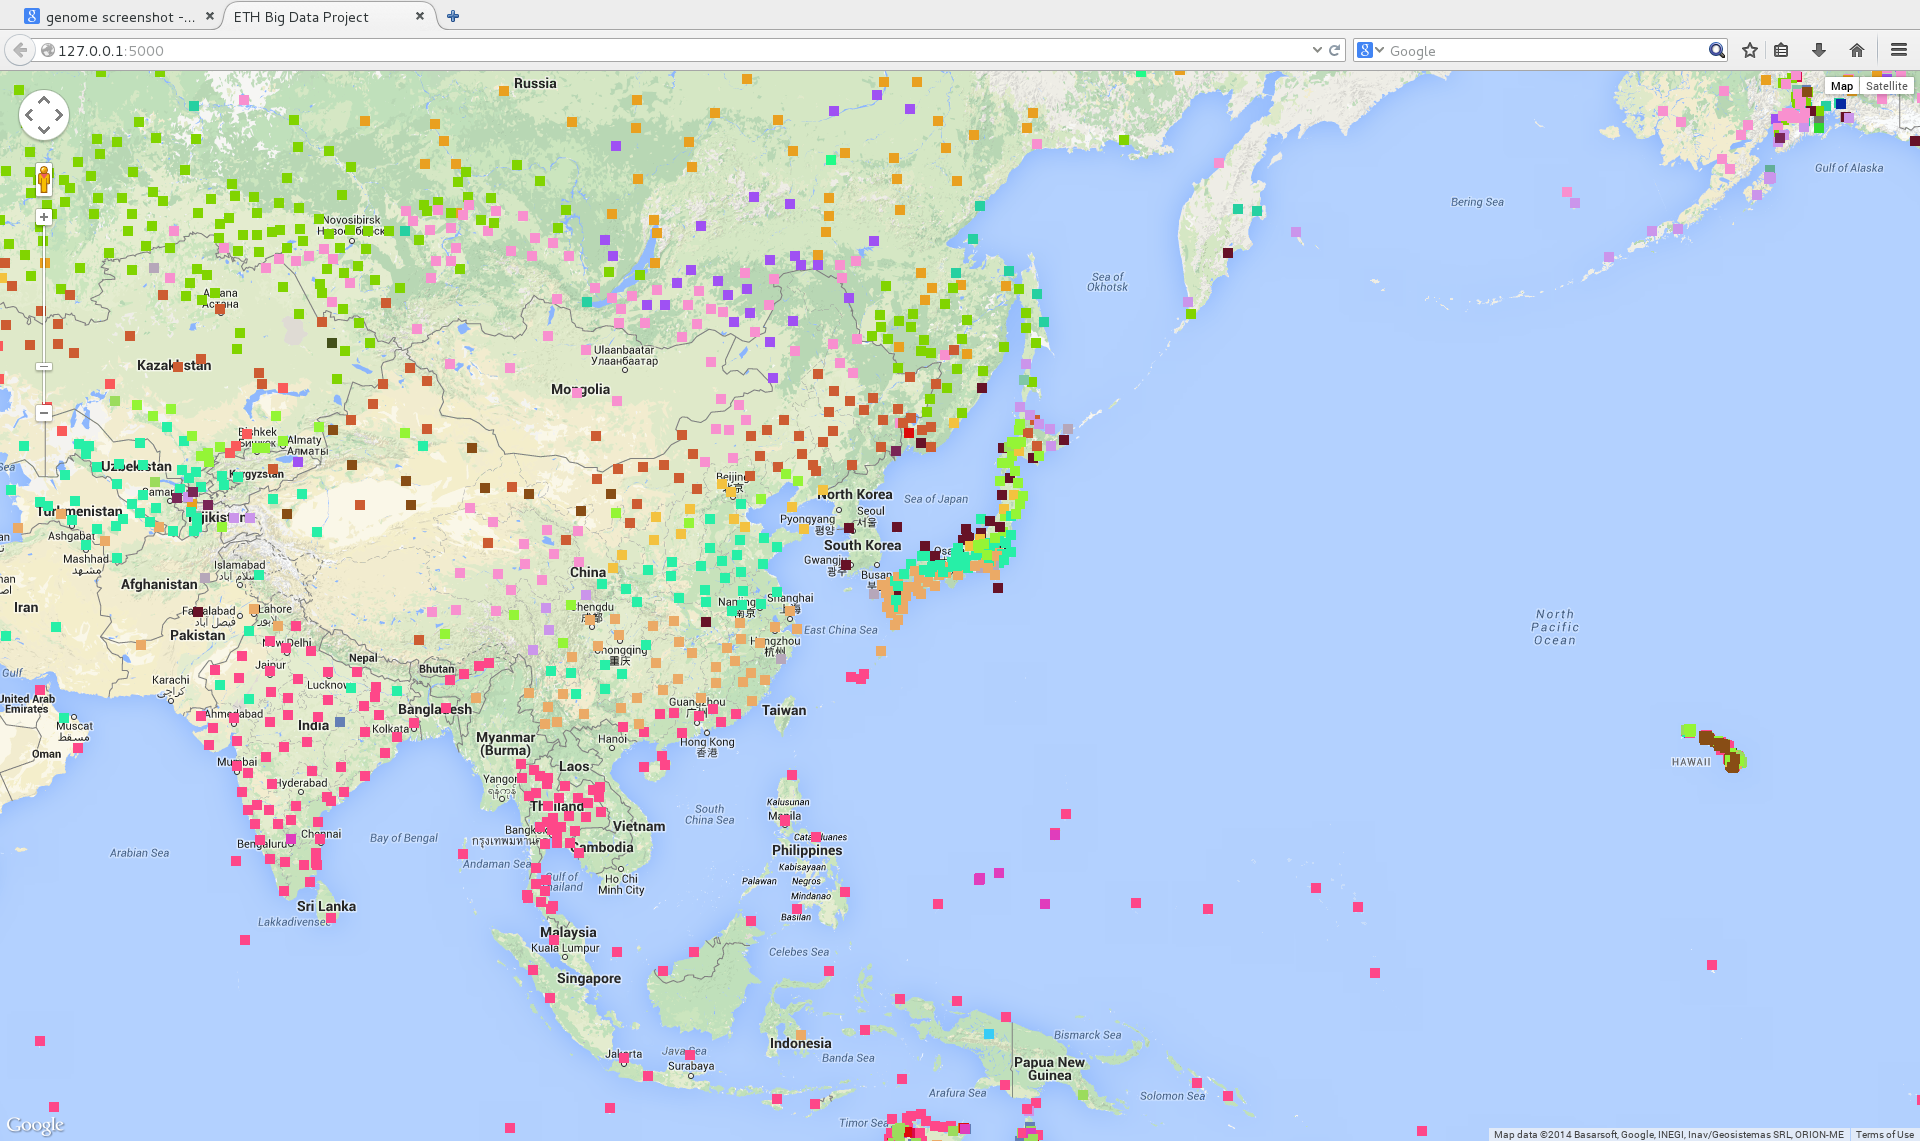
\includegraphics[width=.45\linewidth]{./figure/Ave_60_comp_50_clu_Asia.png}
    \end{tabular}
    \label{fig:AsiaUSAVer}
    \caption{Left: Climate pattern clustering for North American Continent with 75 clusters. Right: Climate pattern clustering for Asia with 50 clusters.}
\end{figure}

As the climate pattern of North America shown in Fig. \ref{fig:AsiaUSAVer}, we can observe an obvious division of Areas closer to the Pacific Ocean and Atlantic Ocean. It is possibly a direct consequence of the different monsoon pattern which are closely related to the two oceans. With closer observation, we can identify three finer-grain clusters. Around Florida, a cluster is formed for the perfect climate pattern of costal vacations. Around the Great Lakes, on the contrary, we observe an patterns which corresponds to extremely code weather in winters. In addition, the light pink region near Nevada surrounded by deep pink patterns reveals the existence of dry climate in desert areas.

In the visualization of Asia climate patterns, we can observe a large cluster of tropical and subtropical climates on South Asia subcontinent and Southeast Asia. Other climate clusters, which distribute in alignment with different latitude range, can be analogously identified. Interestingly, we can observe a three-step structure starting from Chinese coast towards inland of Asia-Europe Continent. The steps corresponds to costal areas, inland plains and inland plateaus, which well explained the variation of height above sea level.



